\section{Vorgehen}

In dem folgenden Abschnitt wird das Vorgehen der Projektgruppe zur Realisierung des Alarmszenarios erläutert. Hierzu wird auf den Arbeitsmodus  und erarbeitete Arbeitsergebnisse eingegangen.

Die Zielsetzung der Projektarbeit \textit{Alaarm-ZIP} lag in der Schaffung eines interaktiven Alarmsimulation, in welcher Übungsteilnehmer fiktive Alarmszenarien im Kontext einer vernetzten Industrie 4.0 Anlage durchlaufen. Die Szenarien werden durch Effekte wie dem Leuchten einer LED-Lampe realisiert, welche beim Übungsteilnehmer einen immersiven Effekt hervorrufen sollen. 

Um die Zielsetzung des Projektes zu realisieren, wurde zum Start des Projektes in der siebenköpfigen Projektgruppe zunächst Themen der Projektorganisation, etwa der Arbeitsmodus und die eingesetzen Tools zum Projektmanagement, festgelegt. Es wurde ein wöchentlicher Sync-Termin mit der Länge von 1 Stunde etabliert. Dieser Termin diente zur gemeinsamen Diskussion der Ergebnisse der vorausgegangenen Woche, der Definition und Festlegung neuer Arbeitspakete für die kommende Woche und der Abstimmung von Terminen in Präsenz zur Erarbeitung größerer Aufgaben von besonderer Bedeutung für den Projektfortschritt. An den Projektstart schloss in der darauffolgenden Woche ein Präsenztermin an, um mithilfe von erarbeiteten Rechercheergebnissen zu verwandten Themen von Alarmszenarien und -simulationen die eigene Aufgabenstellung mittels Brainstorming zu vertiefen. Die Ergebnisse wurden als Mindmap mit dem Kollaborationstool Miro festgehalten. Daran anschließend wurden konkrete Szenarioideen gebildet, welche Gedanken zu Ablauf, Immersionsgeräten und der Administration des Alarmszenarios beinhalten. 

Auf Grundlage der bisher erarbeiteten Ergebnisse wurde sich als Team auf ein Szenario geeinigt, welches als \textit{Minimal Viable Product} (\textit{MVP}) für die Projektarbeit zu realisieren ist. In einer weiteren Arbeitssitzung in Präsenz wurden nun ein Ablaufdiagramm des MVPs in der Prozessmodellierungssprache \textit{BPMN} entwickelt. Unter Abstimmung des aufgestellten Modells mit der Projektleitung von Seiten des Lehrstuhls wurden die technischen Rahmenbedingungen diskutiert. Durch diese Sitzung wurden schlussendlich die technische Implementierung realisiert, um das MVP-Szenario in der Simulationsumgebung des Zentrums Industrie 4.0 am Lehrstuhl für Wirtschaftsinformatik, Prozesse und Systeme der Universität Potsdam zu integrieren. Über den Projektzeitraum hinweg wurde kontinuierlich die hiermit vorliegende Projektdokumentation aktualisiert und weitere Dokumente, wie Beschreibungskarten und Sicherheitsdokumente zur Verwendung für die Alarmsimulation geschaffen.   



\begin{comment}
\section{Beschreibungskarte}


\ 

\textbf{AGENDA} 

\ 

\textbf{3.1 Einleitung und Szenario-Überblick} 
\begin{itemize}
\item
Präsentation des Szenarios und seiner Komponenten
\item
Erklärung des Ablaufs und der Eskalationsstufen
\end{itemize}

\

\textbf{3.2 Sicherheitsbriefing} 
\begin{itemize}
\item
Durchsicht der Gesundheits- und Sicherheitshinweise
\end{itemize}

\

\textbf{3.3 Bedienungsanleitung und Aktivierung der Eskalationsstufe}
\begin{itemize}
\item
Erläuterung der Bedienung der Maschine und des Tablets
\item
Aktivierung der Eskalationsstufe 
\end{itemize}

\

\textbf{3.4 Anzeige der Fehlermeldung und Lösungsansatz }
\begin{itemize}
\item
Erläuterung der Schritte zur Lösung der Fehlermeldungen
\end{itemize}

\

\textbf{3.5 Eskalationsstufe 1}
\begin{itemize}
\item
Durchgehen der Eskalationsstufe 1 und der damit verbundenen Entstörungsvorgang
\item 
Einschreiten der Zufallsvariable
\item
Diskussion über die möglichen Auswirkungen der Zufallsvariable auf den Ausgang des Szenarios
\end{itemize}

\

\textbf{3.6 Eskalationsstufe 2}
\begin{itemize}
\item
Durchgehen der Eskalationsstufe 2 und der damit verbundenen Entstörungsvorgang
\item
Einschreiten der Zufallsvariable
\item
Diskussion über die möglichen Auswirkungen der Zufallsvariable auf den Ausgang des Szenarios
\end{itemize}

 \

\textbf{3.7 Eskalationsstufe 3}
\begin{itemize}
\item
Durchgehen der Eskalationsstufe 2 und der damit verbundenen Entstörungsvorgang
\item
Einschreiten der Zufallsvariable
\item
Diskussion über die möglichen Auswirkungen der Zufallsvariable auf den Ausgang des Szenarios
\end{itemize}

\

\textbf{3.8 Voraussichtliche Zeitangaben des Szenarios zum Abschluss}
\begin{itemize}
\item
Messung der Durchlaufzeit bei optimalen Abläufen
\end{itemize}

\newpage

\subsection{Einleitung und Szenario-Überblick}

In diesem Szenario wird ein komplexes System aus verschiedenen Komponenten und Prozessen beschrieben, das in einen Maschinen-Simulationsraum implementiert wird. Die Szenariokomponenten bestehen aus den Teilnehmern, Tablet, Subwoofer/Lautsprecher, Wärmelampe/Licht und Nebelmaschine. Diese Komponenten sind in einer Umgebung platziert, in der es Anlagen zum Bedienen gibt, die alle durch ein Förderband miteinander verbunden sind. Das System ist so konzipiert, dass es drei Eskalationsstufen gibt, die nacheinander aktiviert werden können. Jede Eskalationsstufe beinhaltet einen Entstörungsvorgang, der vom Teilnehmer gelöst werden muss. Dabei werden verschiedene Szenariokomponenten aktiviert, um den Prozess zu unterstützen und zu simulieren. Teilnehmer des Szenarios, die bei einem Enstörungsvorgang versagen, werden automatisch zur nächsten Eskalationsstufe befördert, bis sie maximal die Eskalationsstufe 3 erreichen. Während eines Enstörungsvorgangs steht den Teilnehmern dabei nur ein Versuch zur Verfügung. Allerdings haben erfolgreiche Szenarioteilnehmer die Möglichkeit, nach Abschluss einer beliebigen Eskalationsstufe das gesamte Szenario vorzeitig zu beenden. Pro Durchgang führt nur ein Szenarioteilnehmer das Szenario durch. Es gibt einen Betreuer, der diese Vorgänge beobachtet und bei Notfällen einschreitet, jedoch ist er nicht für die gesamten Handlungen im Szenarioprozess eingeplant.

\

\underline{Einleitung zum Szenario:} \\
Der Teilnehmer aktiviert die Anlage mit einem Startknopf auf dem Tablet.\hspace{0pt}\marginpar{\footnotesize{ca. 1 Sek.}}
Es wird das Datenpaket für den Szenarioteilnehmer ausgelesen, woraufhin Anweisungen wie Gesundheitswarnungen oder weitere Verfahren angezeigt werden, die der Teilnehmer lesen soll:
\



\

\underline{Einleitung der Eskalationsstufe 1:}

Die Anlage läuft an. \hspace{0pt}\marginpar{\footnotesize{ca. 8 Sek.}}
Gleichzeitig werden in der ersten Stufe die Szenariokomponenten aktiviert, wie der Subwoofer/Lautsprecher, der einen langsamen pulsierenden Ton erzeugt,\hspace{0pt}\marginpar{\footnotesize{ca. 1 Sek.}} sowie die Wärmelampe/Licht (Andon-Signalleuchte), die an der jeweiligen Maschine aktiviert wird und kontinuierlich leuchtet.
Die Anlage ruckelt und stoppt ihren Arbeitsfluss. \hspace{0pt}\marginpar{\footnotesize{ca. 5 Sek.}}

\

\subsection{Anzeige der Fehlermeldung und Lösungsansatz}

\hspace{0pt}\marginpar{\footnotesize{ca. 40 Sek.}} Auf dem Tablet erscheint der Name der betroffenen Maschine, zu der der Szenarioteilnehmer hinlaufen muss:

\

\emph{FEHLERCODE: Machine01}\\
\\

Hinlaufen zu dieser Maschine. \hspace{0pt}\marginpar{\footnotesize{ca. 15 Sek.}}



\



\\
\hspace{0pt}\marginpar{\footnotesize{ca. 45 Sek.}}Auf dem Tablet erscheint ein QR-Code, der gescannt werden muss, um einen Entstörungsvorgang in 40 Sekunden bzw. das Problem zu lösen wie:\

\

Ein großer Button in der Mitte mit der Aufschrift: "Mit Maschine interagieren". \
Der Button verschwindet und macht Platz für den QR-Code-Leser, der wie ein rechteckiges Fenster in der Mitte des Bildschirms erscheint. Wenn der gescannte Code dem erwarteten Code entspricht: Eine Nachricht wird angezeigt, die besagt: "Dies ist der richtige Code! Starte Spiel...".
Wenn der gescannte Code nicht dem erwarteten Code entspricht: Eine rote Fehlermeldung wird angezeigt, die besagt: "Falscher Code! Gehen Sie zu Machine03." Nach einer kurzen Verzögerung von 2 Sekunden wird der QR-Code-Leser erneut aktiviert, um einen weiteren Scan zu ermöglichen.
\



\\


\subsection{Eskalationsstufe 1}


\

\underline{\emph{Numbers-basic}} \\
\emph{Auf dem Tablet wird eine Notiz angezeigt:} \\

\

\emph{(!) Die Werkschritt-Reihenfolge der Maschine scheinen durcheinander gebracht zu sein. } \\

\emph{Klicke auf die Nummern 1 bis 10 in aufsteigender Reihenfolge, um die richtige Reihenfolge wiederherzustellen. Für die Operation sind nur 10 Sekunden vorgesehen!} \\

\emph{3, 5, 8, 10, 9, 2, 7, 4, 1, 6} \\

\


Es folgt eine Verzweigung, die eine Zufallsvariable beinhaltet:

{Nach erfolgreichem Abschluss des Entstörungsvorgangs wird auf dem Tablet eine Benachrichtigung angezeigt, die den Abschluss des Vorgangs bestätigt. Um die Wahrscheinlichkeit von 33\% zu simulieren, wird eine digitale Würfelfunktion verwendet, die die Zahlen 1, 2 und 3 generiert und damit drei mögliche Zustände repräsentiert. Nach dem Entstörungsvorgang wird die digitale Würfelfunktion ausgeführt. Wenn die gewürfelte Zahl eine 1 oder 2 ist (entspricht einer Wahrscheinlichkeit von 2/3), wird auf dem Tablet angezeigt, dass das Problem als gelöst erfasst wurde. Falls die gewürfelte Zahl eine 3 ist (entspricht einer Wahrscheinlichkeit von 1/3), wird auf dem Tablet angezeigt, dass das Problem nicht vollständig gelöst wurde. \\

\begin{itemize}
\item
Sollte der Entstörungsvorgang innerhalb der vorgegebenen Zeit nicht erfolgreich abgeschlossen werden oder eine falsche Eingabe getätigt werden, erfolgt der Übergang zur zweiten Eskalationsstufe automatisch.
\item
Ist der Entstörungsvorgang erfolgreich gelöst, folgt die Zufallsvariable, dabei wird bei einer 1/3 Wahrscheinlichkeit das Problem als nicht gelöst erfasst. Dann erfolgt ebenfalls der Übergang zur zweiten Eskalationsstufe automatisch.
\item
\hspace{0pt}\marginpar{\footnotesize{ca. 3 Sek.}}Wenn der Entstörungsvorgang erfolgreich gelöst ist, folgt die Zufallsvariable, bei der mit einer Wahrscheinlichkeit von 2/3 das Problem als gelöst erfasst wird. Wenn dieses Szenario eintrifft, werden alle Szenariokomponenten ausgeschaltet und das Szenario für den Teilnehmer ist erfolgreich beendet.
\end{itemize}


\newpage 

\subsection{Eskalationsstufe 2}

Simultan werden die Szenariokompontenten Subwoofer/Lautprecher mit einem mittelschnell schlagenden Ton aktiviert. Der Vaporizer stößt derweil Brandgeruch aus. Die LED-Leuchte flackert bei der Maschine blau. Diese bleiben durchgehend in der zweiten Eskalationsstufe aktiv.\hspace{0pt}\marginpar{\footnotesize{ca. 5 Sek.}} \\
Der Szenarioteilnehmer soll sich selbstständig zur nächsten Maschine bewegen, was durch eine Andon-Signalleuchte an der Maschine signalisiert wird. (Zeit: ca. 15 Sekunden) \\
\hspace{0pt}\marginpar{\footnotesize{ca. 40 Sek.}}Erneut muss ein Entstörungsvorgang durchgeführt werden: 

\

\underline{\emph{Reaction}} \\
\emph{(!) Auf dem Tablet wird eine Notiz angezeigt:}\\

Problem mit der Kalibrierung! Etwas scheint mit der Kalibrierung der Maschine ein Problem zu geben, das schwerwiegende Fehler auslöst. Um alle möglichen Fehlerquellen auszuschließen, müssen die Eingaben neu kalibriert werden. \\
          
Zur korrekten Kalibrierung muss der richtige grün aufleuchtende Bereich innerhalb von 0,6 Sekunden gedrückt werden. Die Bereiche fangen in einem schwarzen Zustand an. Falls du länger als 0,6 Sekunden brauchst, um den grün aufleuchtenden Bereich zu drücken, kann die Maschine nicht kalibriert werden. Es benötigt 6 erfolgreiche Kalibrierungen.

\

\includegraphics[width=1.6cm, height=1.3cm]{res/2cube.jpg} \\
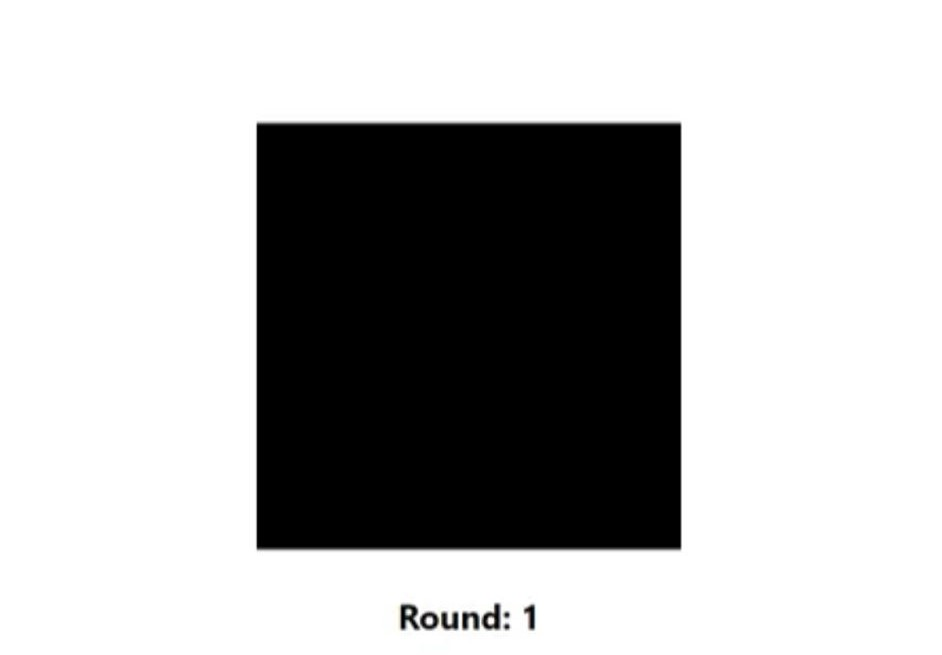
\includegraphics[width=3cm, height=2cm,]{res/cube.jpg} 


\

Danach erfolgt eine weitere Verzweigung, bei der die Zufallsvariable aktiviert wird. \\

\

\subsection{Eskalationsstufe 3} \\

Gleichzeitig werden die Szenariokomponenten Subwoofer/Lautsprecher mit einem schnell schlagenden Ton, der Vaporizer mit einem intensiveren Geruch als zuvor und die Wärmelampe aktiviert. Die Andon-leuchte flackert rot. Diese bleiben durchgehend in der dritten Eskalationsstufe aktiv.\hspace{0pt}\marginpar{\footnotesize{ca. 5 Sek.}} \\
Der Szenarioteilnehmer soll zur nächsten Maschine, welches durch eine Andon-Signalleuchte signalisiert wird, hinbewegen.\hspace{0pt}\marginpar{\footnotesize{ca. 15 Sek.}} \\
Erneut muss ein Entstörungsvorgang durchgeführt werden: \hspace{0pt}\marginpar{\footnotesize{ca. 40 Sek.}}

\

\underline{\emph{Numbers-advanced}} \\
\emph{Auf dem Tablet wird eine Notiz angezeigt:} \\

\

\emph{(!) Die Werkschritt-Reihenfolge der Maschine scheinen durcheinander gebracht zu sein. } \\

\emph{Der Algorithmus der Maschine scheint ein Problem zu haben. Mehrere Prozesse scheinen separat zu laufen, die wieder in die richtige Reihenfolge gebracht werden müssen.
        Klicke die Nummern 1 bis 10 in aufsteigender Reihenfolge an, um dies zu tun.
        Nach jeweils 5 und 10 Sekunden werden die Zahlen gemischt.
        Für diese Reparatur sind lediglich 15 Sekunden vorgesehen!} \\


\emph{3\hspace{15pt} 5\hspace{42pt} 8\hspace{58pt} 10\hspace{75pt} \\9\hspace{25pt} 2\hspace{37pt} 7\hspace{83pt} \\4\hspace{39pt} 1\hspace{66pt} 6\hspace{81pt}} \\

\
Danach erfolgt eine weitere Verzweigung, bei der die Zufallsvariable aktiviert wird.

\

\subsection{Voraussichtliche Zeitangaben des Szenarios}
Sämtliche Zeitangangaben beruhen auf einer Schätzung bzw. theoretischen Planung und sind je nach individueller Durchführung und Reaktionsgeschwindigkeit des Teilnehmers variabel. Diese Zeitangaben stehen daher unter Vorbehalt und dienen lediglich als grobe Orientierung. Es ist möglich, dass die tatsächliche Dauer für jeden Teilnehmer unterschiedlich ist. \\

\

\underline{Benötigte Zeit für Eskalationsstufe 1} \\
Lesen der Anweisungen: ca. 2 Minuten \\
Aktivierung der Anlage: ca. 8 Sekunden \\
Unterbrechung der Anlage ca. 5 Sekunden \\
Anzeige der Fehlermeldung: ca. 40 Sekunden \\
Hinlaufen zur Maschine: ca. 15 Sekunden \\
Entstörungsvorgang in der ersten Stufe: ca. 45 Sekunden \\
Einschreiten der Zufallsvariable: ca. 3 Sekunden \\
Geschätzte Gesamtzeit für den Abschluss der ersten Stufe: ca. 4 Minuten \\

\

\underline{Benötigte Zeit für Eskalationsstufe 2} \\
Zeit für die erste Stufe: ca. 4 Minuten \\
Hinlaufen zur Maschine: ca. 15 Sekunden \\
Entstörungsvorgang in der zweiten Stufe: ca. 40 Sekunden \\
Einschreiten der Zufallsvariable: ca. 3 Sekunden \\
Geschätzte Gesamtzeit für den Abschluss der ersten und der zweiten Stufe: ca. 5 Minuten \\

\

\underline{Benötigte Zeit für Eskalationsstufe 3 / Max. Zeit bei Erfolglosigkeit} \\
Zeit für die zweite Stufe: ca. 5 Minuten \\
Hinlaufen zur Maschine: ca. 15 Sekunden \\
Entstörungsvorgang in der dritten Stufe: ca. 40 Sekunden \\
Einschreiten der Zufallsvariable: ca. 3 Sekunden \\
Geschätzte Gesamtzeit für den Abschluss der ersten, zweiten und der dritten Stufe: ca. 6 Minuten \\
\end{comment}



